\section{GPU占用率与延迟隐藏技术详解}

\subsection{引言：占用率的概念区分}

本章将深入探讨占用率（Occupancy）和利用率这两个概念，即比较不同架构时所需的关键参数。本章开头有必要重温课程中一个重要章节的内容——讨论了一系列关键参数，如内存带宽和指令吞吐量。在本章中，将引入占用率作为另一个评估性能的关键术语。

这个术语的真正问题在于，大多数涉及该主题的教程倾向于只解释理论占用率，而不是实际达到的占用率。GPU 的占用率是衡量 GPU 中资源利用率的一个指标。在 GPU 性能领域，占用率被分为两种不同的类型：理论占用率代表理想化场景，达到的占用率表示 GPU 资源的实际使用情况。

理论占用率的计算方法是将核函数中使用的 Warp 数除以每个 SM（流式多处理器）所能容纳的最大 Warp 数。这里涉及两个关键值：分子根据应用程序中使用的 Warp 数而变化；分母对应 GPU 的 Warp 数限制，这个限制可以从 GPU 白皮书中获取，或者使用前文介绍的运行时 API 获取。

\subsection{获取硬件限制：运行时API示例}

\begin{figure}
    \centering
    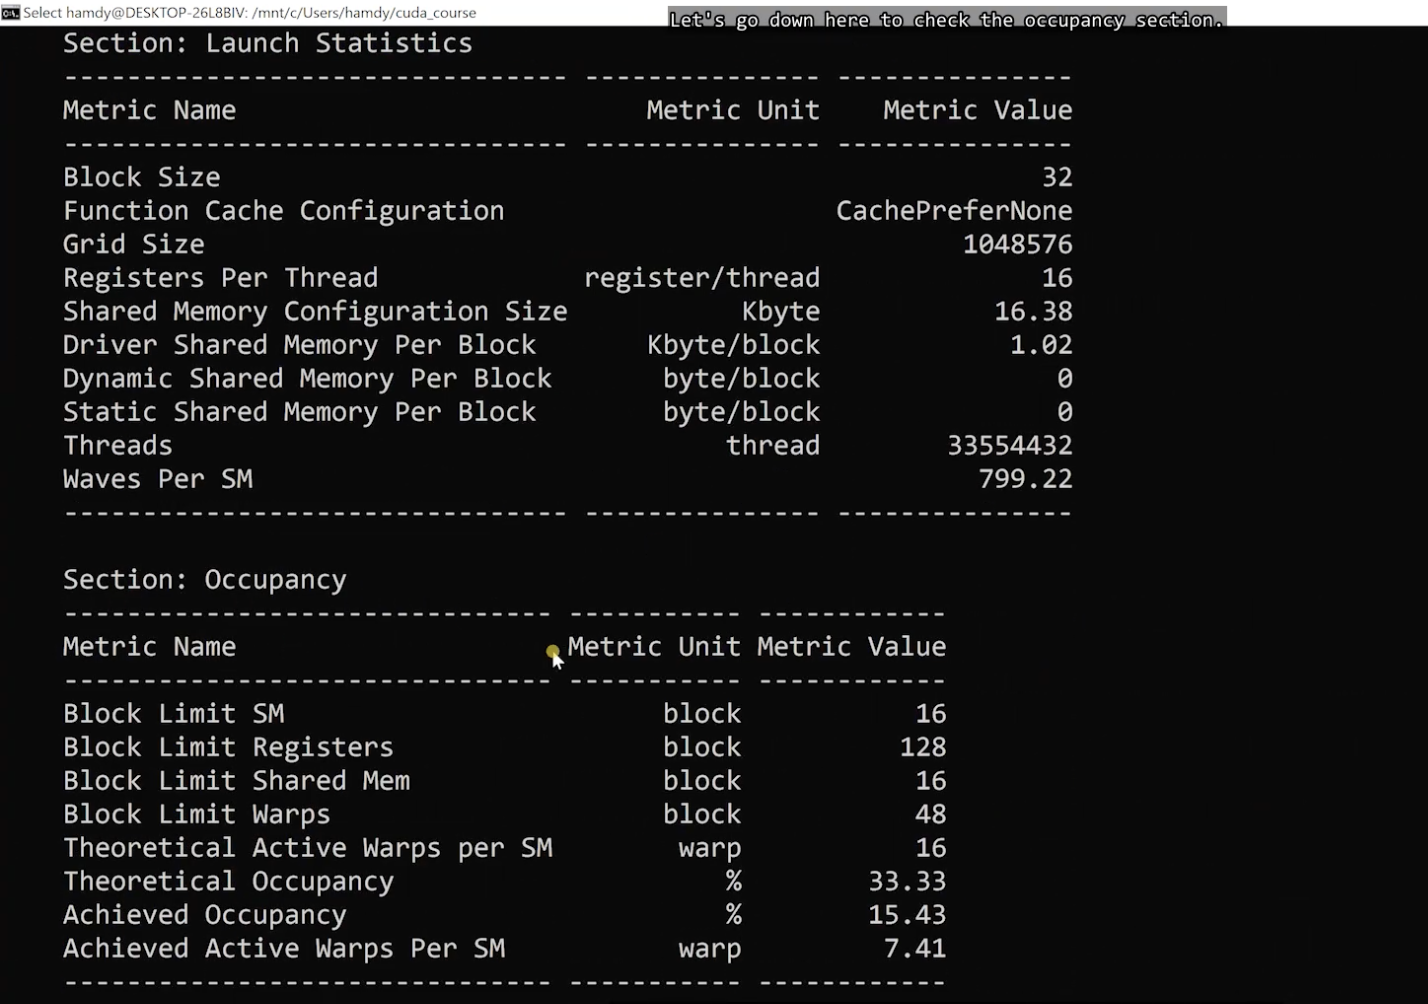
\includegraphics[width=0.75\linewidth]{resources/cuda-091.png}
    \caption{}
    \label{fig:placeholder}
\end{figure}

运行一个简单的代码，它包含运行时 API 函数，用于获取 GPU 每个 SM 的最大 Warp 数。首先使用 \texttt{nvidia-smi} 命令来识别 GPU 的名称，以获取方程的分母。如输出所示，GPU 是 GeForce 系列的一员，具体型号是 RTX 3090。

既然已经确定了正在处理的是哪个 GPU，现在把注意力转向代码，类似于前文的方法。从 \texttt{cudaGetDeviceCount} 函数开始，它提供系统中可用的支持 CUDA 的 GPU 总数。如果有两块 NVIDIA GPU 和一块 AMD GPU，AMD GPU 将不会包含在此变量中，即该变量只会包含 2 而不是 3。

然后使用 \texttt{cudaDeviceProp} 结构体来创建对象，用于存储所选 GPU 的所有属性。如果只有一个 GPU，使用索引 0 即可，无需使用 for 循环遍历所有 GPU。这里的 \texttt{cudaGetDeviceProperties} 函数读取 GPU 的所有属性，从 GPU ID=0 读取的属性将被存储在这个对象中。

这里打印的是每个 SM 的最大 Warp 数。如果想打印此对象中的任何度量指标，需要使用点运算符。例如 \texttt{prop.maxThreadsPerMultiProcessor} 获取每个 SM 的最大线程数，再除以 32 即可得到最大 Warp 数，因为每个 Warp 包含 32 个线程。

还有另一种读取这些度量指标的方法，涉及使用 \texttt{cudaDeviceGetAttribute} 函数。从其名称可知，此函数可用于从任何设备读取单个属性。例如在这种情况下，需要读取每个 SM 的最大 Warp 数，只需写入属性的名称，属性名称可以在该函数的文档中查到。

在文档中搜索该函数，它接受三个参数：第一个是值（存储结果），第二个是度量指标或属性的名称，最后一个是设备 ID。如果计算机中有多个 GPU，需要确定是从 GPU ID=0 还是 ID=1 或 ID=2 读取。如所示，有几十个可以读取的属性，例如每个块的最大寄存器数、多处理器数量、ECC 错误纠正、内存时钟频率等。前文已通过 \texttt{nvidia-smi} 命令检查过内存时钟频率，这里是读取它的另一种方法。

这里需要的度量指标是 \texttt{cudaDevAttrMaxThreadsPerMultiProcessor}。这个函数需要两个输入：设备 ID 和属性名称，然后属性值将被存储在定义为整数的变量中。同时可以将该值除以 32 以获得每个 SM 的最大 Warp 数。

进入 CUDA 课程文件夹，列出所有可用文件。复制文件名，然后使用 nvcc 编译器，将可执行文件命名为 \texttt{read\_metrics}，放上 \texttt{.cu} 文件，点击回车。执行后，如所示，RTX 3090 GPU 中每个 SM 的最大 Warp 数是 48（1536/32）。使用第二个函数结果也一样，两种方法都可以使用。

\subsection{理论占用率计算示例}

现在已知每个 SM 的最大 Warp 数是 48。看一些例子来理解理论占用率。

在第一个场景中，考虑一个设计为使用每个 SM 48 个 Warp 的 CUDA 应用程序。计算比率得出理论占用率为 100\%，因为应用程序中使用的 48 个 Warp 与每个 SM 的 Warp 上限 48 相匹配。

在第二个场景中，如果应用程序配置为使用每个 SM 12 个 Warp，那么 $12/48$ 的比率表明理论占用率降低到了 25\%。然而在后续两个章节中，将探讨更复杂的场景。因为占用率与另一个称为"每个 SM 分配的活动块"的术语有关，该术语将在后续章节中探讨，这里只是简化的例子。

\subsection{向量加法案例研究}

\begin{figure}
    \centering
    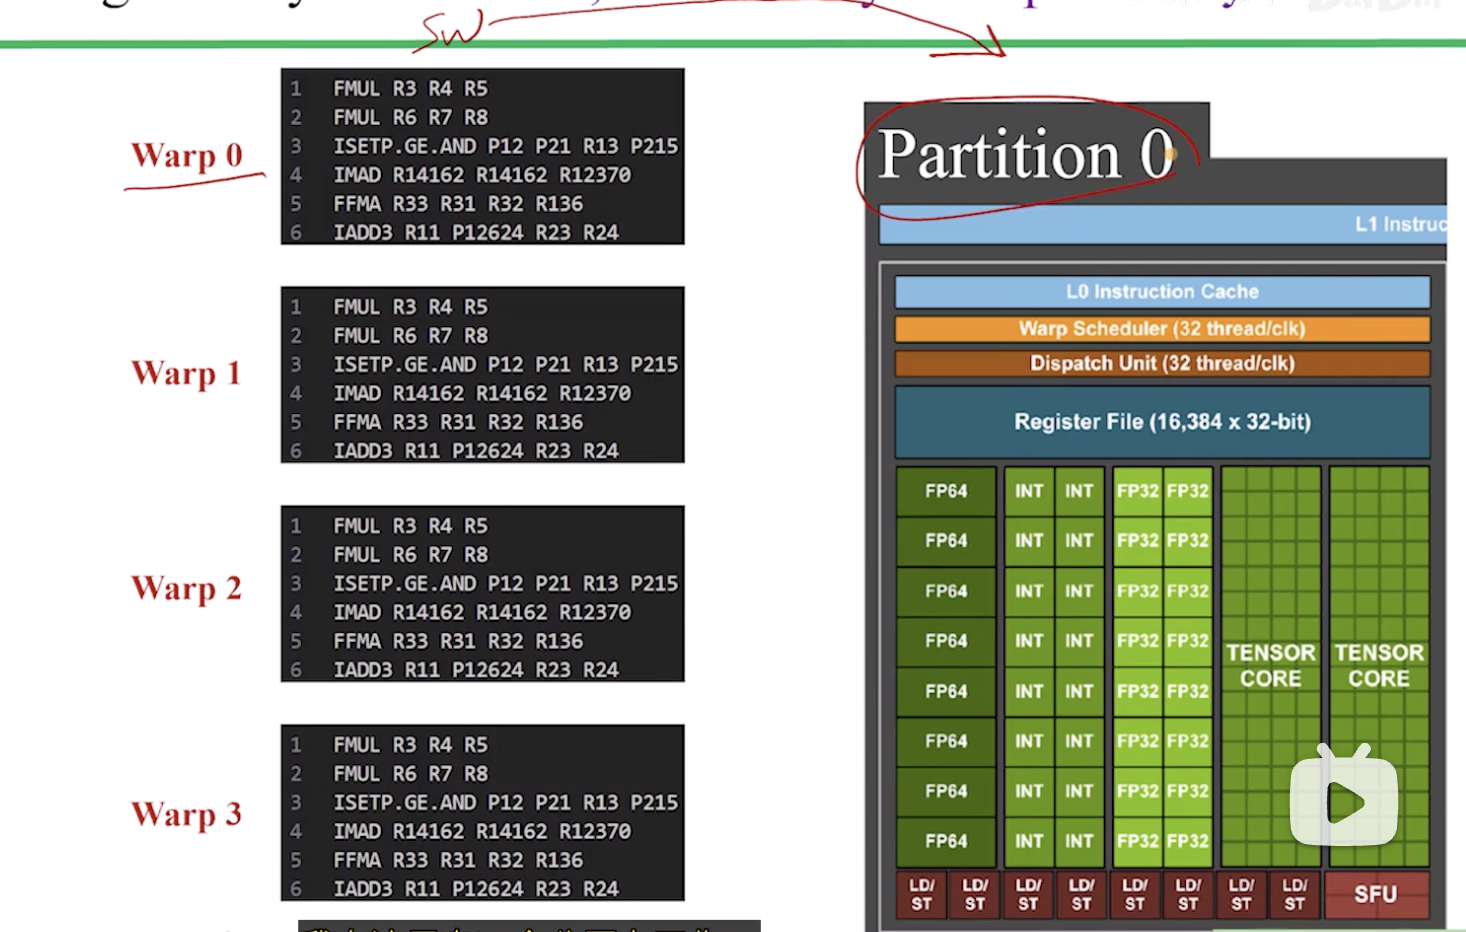
\includegraphics[width=0.75\linewidth]{resources/cuda-092.png}
    \caption{}
    \label{fig:placeholder}
\end{figure}

深入评估与向量加法应用相关的理论占用率。本章的主要目的是专注于占用率这个术语，因此不会解释 Nsight Compute 工具中的不同选项，仅使用最简单的命令。

列出文件夹中所有的 CUDA 文件，复制向量加法文件并进行编译：\texttt{nvcc -o vector\_add vector\_add.cu}。如所示，它正确执行了，执行时间大约为 6.5 毫秒。

需要分析这个应用，可以使用 \texttt{ncu} 命令（即 Nsight Compute）。如所示，分析过程已启动。从头开始看：核函数名称是 \texttt{vectorAdd}，这些是核函数的输入参数和维度。可以从 CUDA 文件本身读取这些值：每个块的线程数是 32，块的总数是通过方程计算得出的。

往下滚动到占用率部分。有 SM 块限制、寄存器块限制、共享内存块限制、Warp 块限制等参数，这些将在后续章节中解释。然后是理论上的每个 SM 活动 Warp 数和理论占用率。如所示，理论占用率是 33.33\%，意味着只使用了 GPU 总可用资源的三分之一。即使往下查看达到的占用率，有更低的值，这意味着在实际执行中，只使用了理论占用率的一半。

这就是为什么选择每个块的线程数对于应用程序的占用率非常重要。举例来说，把这个值增加到 64，看看改变它将如何影响占用率。重新编译并重新分析。理论占用率翻倍了，达到的占用率也从 15\% 增加到了 51\%。理论占用率现在是 66.67\%。

为什么改变每个块的线程数会增加理论和达到的占用率？关注理论占用率：看这些限制值，取最小值，现在是 16。这意味着将在每个 SM 上同时执行 16 个块。块大小是指每个块的线程数，取这两个值相乘：$64 \times 16 = 1024$ 个线程。除以 32 得到 32 个 Warp。已知最大值是 48，所以 $32/48 = 66.67\%$。

以上展示了如何获得理论占用率。同时也解释了为什么这个值影响了理论占用率：因为它将每个块的 Warp 数从 1 个增加到了 2 个（64 线程 = 2 个 Warp）。

再将这个值增加到 96。不能写 100，因为 100 意味着 4 个 Warp（即使选择 100 个线程，也将执行 128 个，因为这取决于有多少个 Warp）。重新编译并重新分析。可以计算那种情况下的理论占用率：每个块 96 线程 = 3 个 Warp，最小值仍然是 16 个并发块，$3 \times 16 = 48$ 个 Warp，这与每个 SM 的最大 Warp 数相同，意味着理论占用率是 100\%。

如果查看结果，理论占用率确实是 100\%，然而达到的占用率大约为 73\%。这就引出了接下来要解释的内容：为什么这两个值之间有差异。

\subsection{理论占用率总结}

总之，理论占用率指的是在理想情况下核函数可以使用的 GPU 计算资源的最大百分比。这里讨论的是理想情况，它被称为理论的而不是实际的，因为它假设了最优条件：既有足够的独立任务或足够的线程来完全占用 GPU 的资源，而不受内存/计算指令间依赖或同步约束的瓶颈影响。

\subsection{达到的占用率与延迟隐藏}

\begin{figure}
    \centering
    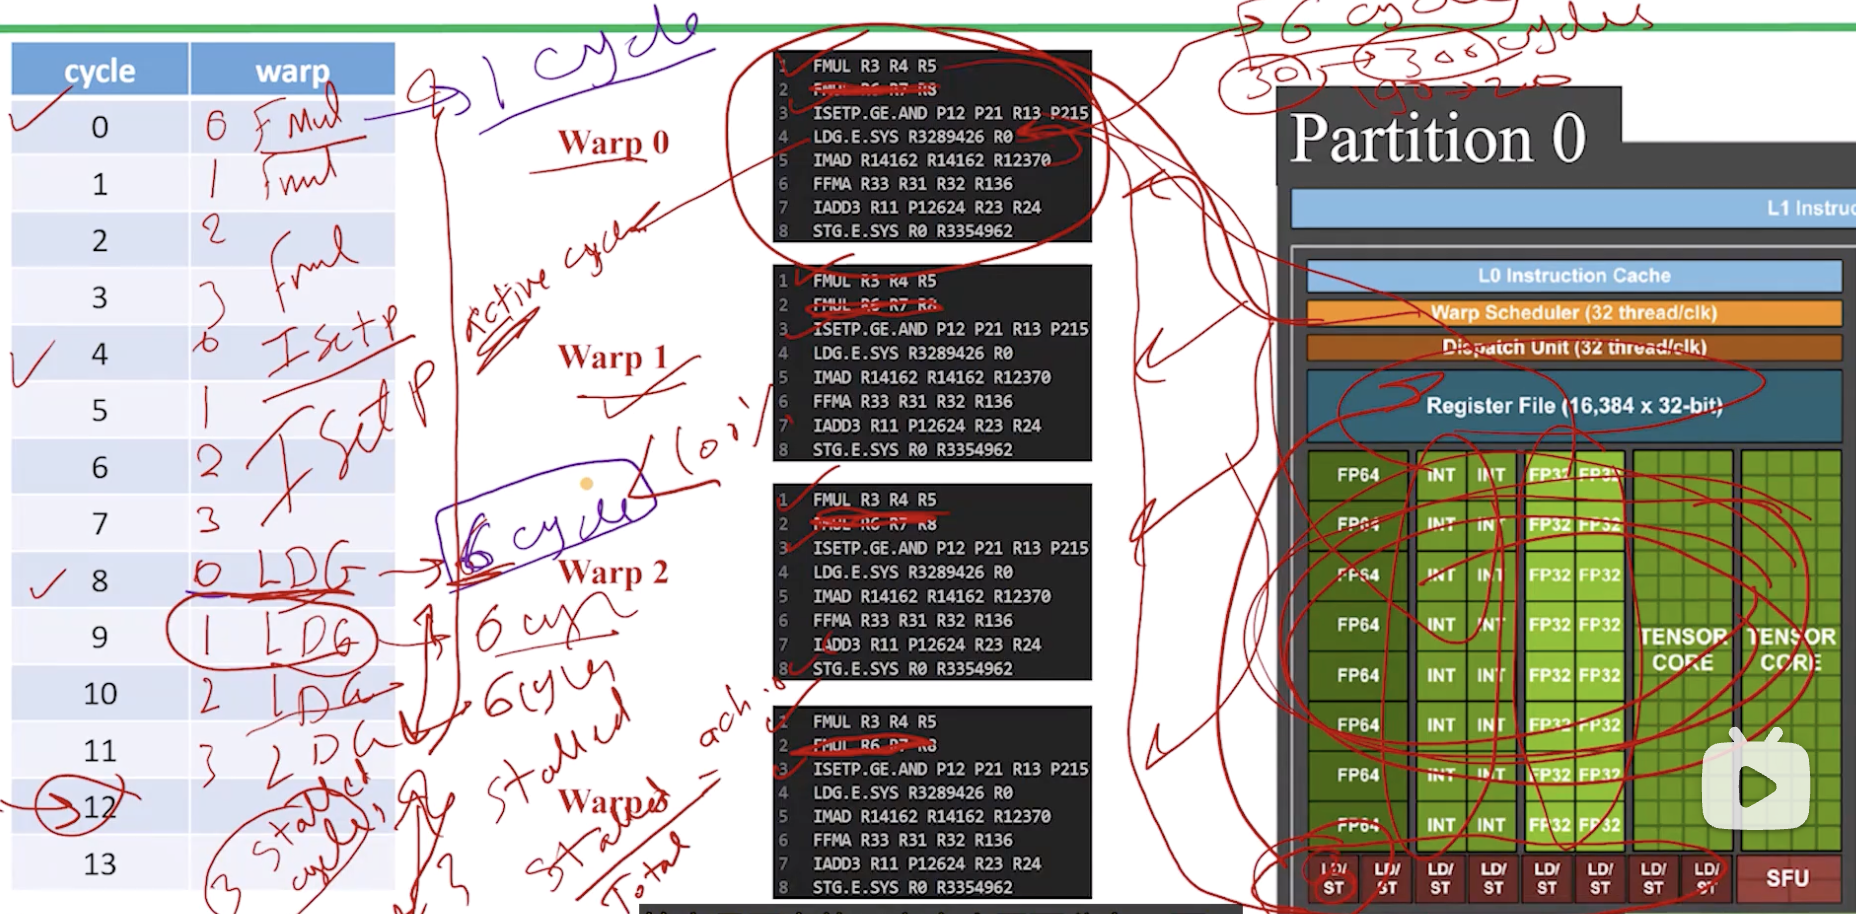
\includegraphics[width=0.75\linewidth]{resources/cuda-093.png}
    \caption{}
    \label{fig:placeholder}
\end{figure}

现在把重点转移到达到的占用率。首先回顾 GPU 的结构：一个 GPU 由多个 SM 组成，每个 SM 包含多个分区。在 Ampere 和 Volta 架构中，每个 SM 包含四个分区。这是一张仅一个分区的图片，在本章剩余内容中会用到它。

在这个层级中，应用程序在整个 GPU 上运行，块被指定在 SM 上运行，而 Warp 在分区上执行。Warp 是本章的焦点，需要来自软件的 Warp 和来自硬件的分区。调度单元负责获取就绪 Warp 的就绪指令，并将它们发送到适当的计算单元。GPU 内的每个分区包含一个调度器，它负责在每个周期分配一个 Warp 来执行。

\subsection{简化示例设定}

假设有一个应用程序，其中每个 SM 只取一个块，并且块大小是 512 个线程。这意味着块大小等于 16 个 Warp（$512/32$）。同时假设使用一个不同的 GPU，其限制是每个 SM 16 个 Warp。$16/16$ 得出的理论占用率为 100\%。

然而对于达到的占用率，存在 Warp 未就绪的情况。例如当一个 Warp 正在等待来自内存的值时，这可能需要 30 到 300 个周期不等，具体取决于访问的缓存级别。在此期间，其他 Warp 可能被调度执行。但如果所有 Warp 都遇到显著的内存请求或指令依赖，调度器可能会遇到没有 Warp 准备好执行的周期，这就引入了所谓的停顿周期（Stall Cycle）。

\subsection{场景一：无内存请求无指令依赖}

有两个场景来澄清这一点。在第一个场景中，假设没有内存请求或指令间的依赖。这里涉及两个术语：占用率和延迟隐藏，将在后面解释。

从这张图片开始，包含了某个代码应用的部分汇编指令。可以使用名为 \texttt{nvbit} 的工具获得这个指令跟踪。在 NVIDIA GPU 的情况下，汇编指令被称为 SASS 指令。可以搜索该工具以了解更多信息，同时也搜索 SASS 指令这个术语。

这张图片仅代表一个 Warp，但假设有四个 Warp。在硬件部分，假设将在一个分区上执行这四个 Warp（不是一个 SM，不是整个 GPU）。请问：每个分区利用了多个 Warp，在这种情况下有四个 Warp，能计算每个 SM 利用的 Warp 数吗？答案是肯定的。如果一个 SM 有四个分区，每个分区执行 4 个 Warp，那么每个 SM 的最大 Warp 总数将是 $4 \times 4 = 16$。

能计算理论占用率吗？理论占用率等于应用程序中使用的 Warp 数除以总数再乘以 100\%。在这种情况下，最大 Warp 数是 16，应用程序中使用的 Warp 总数也是 16，所以理论占用率是 100\%。

下面解释 Warp 调度器的功能。Warp 调度器开始与所有 Warp 对话，询问它们谁准备好执行其指令之一。假设 Warp 0 会说："是的，我准备好执行这里的第一个指令，即 FFMA（F 指的是浮点乘法）。"调度器会说是的，有就绪 Warp，它准备好执行 FFMA。调度器将获取这个指令并将其发送到所有这些核心。可能会疑惑为什么取一个指令并发送给所有这些核心，只需要一个核心？答案实际上不止一个指令，有 32 个 FFMA 指令。

为什么有 32 个指令？需要记住每个 Warp 由 32 个线程组成。这些线程执行相同的指令但处理不同的数据，这意味着这个指令后面应该跟着另一个 FFMA 指令用于第二个线程但使用不同的寄存器。对于所有 32 个线程都是如此，这就是为什么这个指令将被获取并发送到这些核心执行。在周期 0 中，拥有就绪 Warp 准备好执行 FFMA 指令。

然后在下一个周期，调度器会再次询问谁准备好执行指令。假设它们按顺序执行，Warp 1 应答并就绪，可以执行第一个 FFMA。调度器将类似于第一个 Warp 那样获取这个指令并发送到核心。对于 Warp 2 和 Warp 3 同样适用。然后这个周期将再次重复，Warp 0 将在周期 4 回复 FFMA 指令。

然后在周期 8，Warp 调度器将再次询问所有 Warp 谁就绪以及什么指令就绪。Warp 0 会说："我就绪了，有一个整数指令 ISETP。"ISETP 是一个用于比较的整数指令，它比较两个值并选择其中一个。比方说如果其中一个大于另一个，它会取第一个并存储在这里；如果不是更大的那个，它会取第二个并存储在这里。在这个例子中它是一个整数指令，调度器会获取这个指令并将其发送到整数流水线。对于所有其他 Warp 也同样适用。

同样的周期再次重复，可以说达到的占用率等于 100\%。为什么？因为每个周期都有一个 Warp 准备好执行它的指令之一。如果出于任何原因，在这些周期中的任何一个发现 Warp 都没有准备好执行，这将被称作一个停顿周期。没有 Warp 就绪意味着停顿周期，在这种情况下达到的占用率将小于 100\%。当指令间没有依赖时，达到的占用率是 100\%，等于理论占用率。

\subsection{延迟隐藏的概念}

但场景一中没有内存请求，这是一个非常简单的例子。下面解释延迟隐藏这个术语。

延迟隐藏是 GPU 相较于 CPU 的主要特性之一。在 CPU 的情况下，没有这么多计算资源，可能有 4 个、8 个或 16 个核心，这就是为什么在 CPU 的情况下没有 Warp。CPU 使用一些技术，例如乱序执行（Out-of-Order Execution）。

举例来说。假设有 \texttt{ADD R1, R2, R3}，然后 \texttt{MUL R4, R1, R5}，再假设有 \texttt{SUB R10, R11, R12}。如果关注前两条指令，可以看到这里有依赖关系：MUL 指令依赖 ADD 指令的结果 R1。

当 ADD 指令进入 CPU 执行时，下个周期不会发送 MUL 指令，因为有依赖关系。MUL 必须等待 ADD 完成然后才开始执行，在这种情况下有一些停顿周期。CPU 使用乱序执行技术：SUB 指令没有依赖，CPU 改变指令顺序使其准备好执行，当 ADD 在执行时 SUB 可以发送给 CPU 准备在下个周期执行。

这可以应用于 CPU，但在 GPU 中不需要那样。为什么？在 GPU 的情况下，大多数时候不止有一个 Warp，有很多 Warp，它们可能包含一些就绪的指令。如果这个 Warp 没有就绪（比如有依赖关系），不需要对指令进行重排序，因为可以和另一个 Warp 对话，通常可以找到一个就绪的指令。这就是所谓的通过提供大量 Warp、大量线程、大量指令在所有计算单元上执行来隐藏延迟。

\subsection{场景二：内存请求与指令依赖}

在第二个场景中，假设只有一个内存请求并且还有一个指令依赖。看看从这个地址读取值并存储到这个寄存器。假设 LDG 指令（全局内存加载）将等待来自内存的值。

在 LDG 指令和后续指令之间存在依赖关系，有一个内存请求和一个依赖。还假设有四个 Warp。假设只有一个 FFMA，在第一个周期调度器询问所有 Warp 谁就绪，第一个 Warp 用 FFMA 回复，调度器获取指令并发送。Warp 0 就绪执行 FFMA。下一个周期 Warp 1 就绪又是 FFMA，Warp 2、Warp 3 同样，前四个周期执行 FFMA，与场景一类似。

假设加载指令将消耗 6 个周期（通常实际值在 30 到 300 个周期之间，取决于访问的缓存级别：L1 缓存约 30 周期，L2 缓存约 190-200 周期，全局内存约 300 周期）。为了简单起见假设 6 个周期。

那么在周期 4 执行完 FFMA 之后，调度器再次与所有 Warp 对话。Warp 0 说准备好执行整数指令 ISETP，调度器将其带到整数单元。Warp 1、2、3 同样适用。在这里完成了 ISSUED。

调度器再次问谁就绪，Warp 0 说准备好了但现在在执行加载指令。在周期 8，加载指令将被调度器移到加载/存储单元（Load/Store Unit），而不是计算单元。加载/存储单元负责内存不同级别（L1、L2、全局内存）之间的连接。这个指令消耗 6 个周期，意味着这个 Warp 将不可用除非 6 个周期结束。

然后 Warp 调度器问第二个 Warp 准备好了吗？它说准备好执行加载指令，但这也要花费 6 个周期。Warp 2 和 3 同样加载 6 个周期。

现在在周期 12，最重要的一点是调度器将与 Warp 0 对话："准备好了吗？"Warp 0 会说："不，还没准备好。因为想执行 ISETP 指令，但这个指令依赖于从内存来的结果，现在没准备好因为加载指令还没完成。"为什么没准备好？这里只过了 3 个周期（从周期 8 到周期 12 是 4 个周期，但加载需要 6 个周期），还必须再等 2 个周期才会准备好。

调度器将询问下一个 Warp，Warp 1 也会说不可用因为加载指令需要 6 个周期还没完成。这就是为什么这里至少会有 2 到 3 个停顿周期。停顿意味着所有这些 Warp 中没有一个准备好执行任何指令，因为内存请求。

在这种情况下可能会看到一些活动周期（Active Cycle），因为在这个周期中计算单元之一是活动的，正在执行 FFMA 或 ISETP 甚至是加载。但这里有停顿的情况。将活动周期除以总周期（而不是停顿周期）将得到达到的占用率。

举一个带数字的例子。假设总共有 100 个周期，有 85 个活动周期，那么将有 15 个停顿周期。达到的占用率等于 $85 / 100 = 85\%$。

现在已知什么是达到的占用率以及它与理论占用率的区别。为什么理论占用率是 100\% 而达到的占用率是 85\%？因为理论占用率只取决于 Warp 的数量，这很容易计算，所以它被称为理论的。但达到的占用率取决于每个 Warp 指令在执行时的动态实时行为。

\subsection{Nsight Compute实测验证}

\begin{figure}
    \centering
    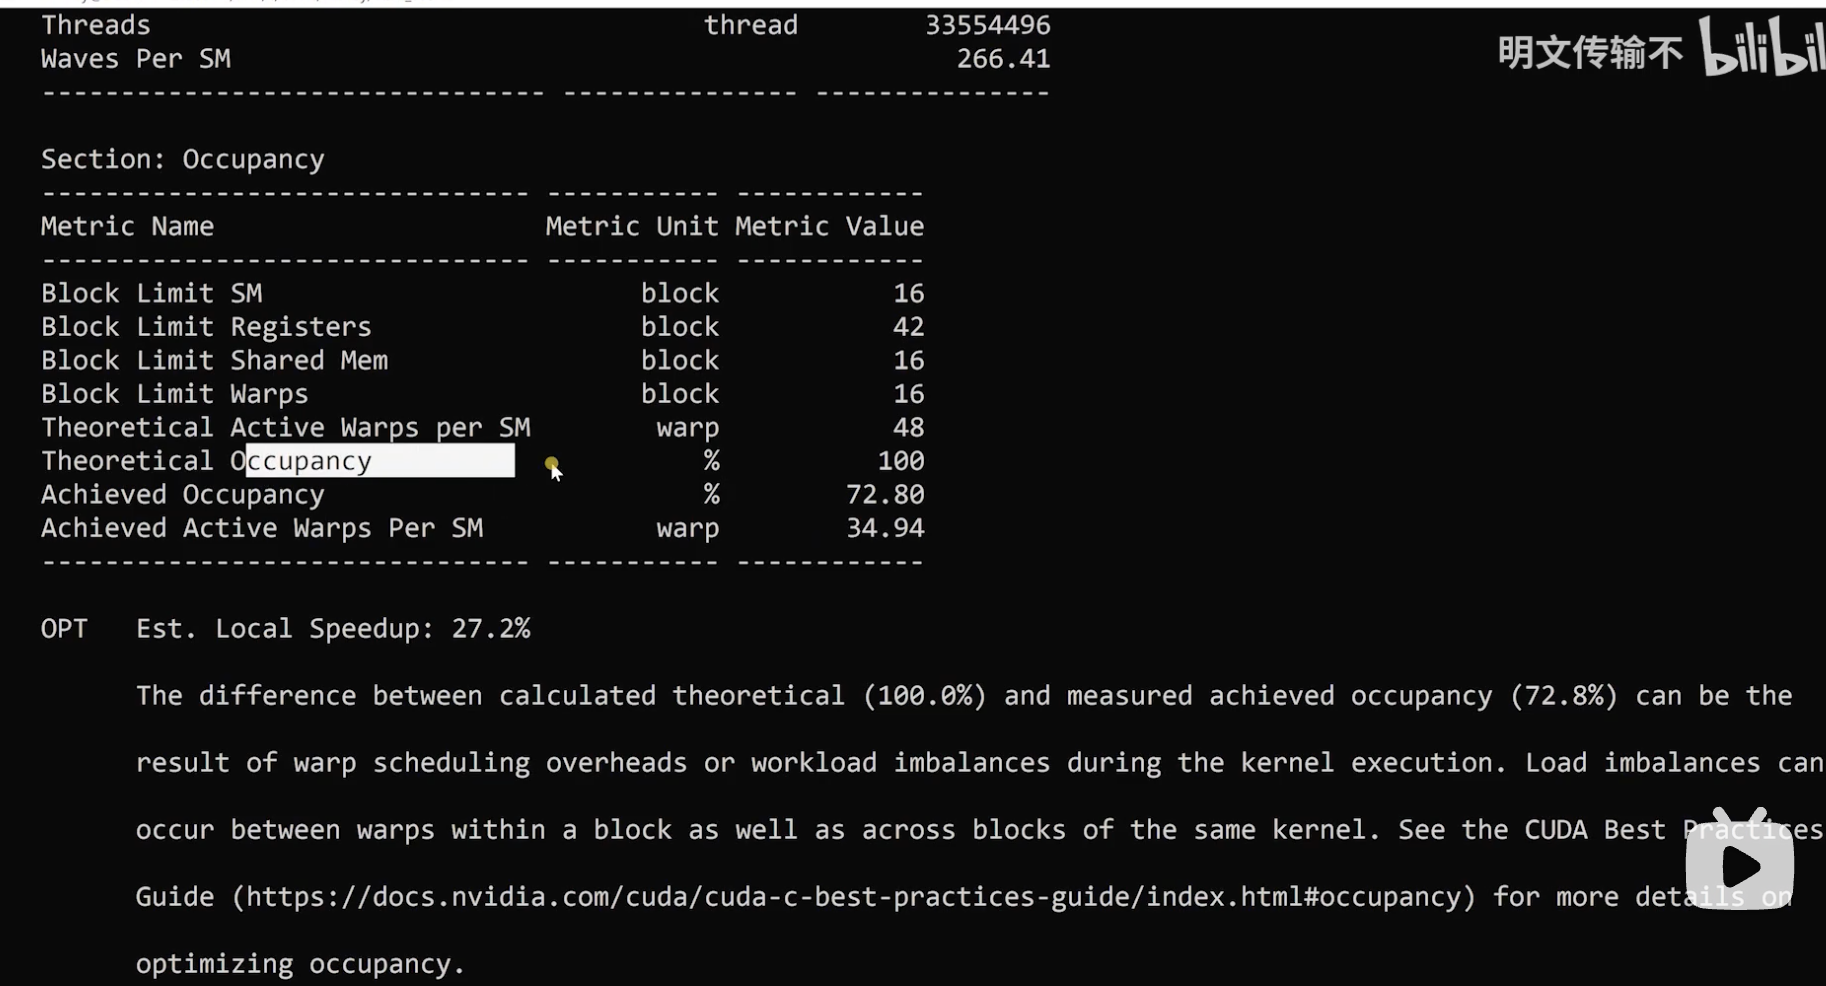
\includegraphics[width=0.75\linewidth]{resources/cuda-094.png}
    \caption{}
    \label{fig:placeholder}
\end{figure}

再次运行 \texttt{ncu ./vector\_add}。达到的占用率是 72.8\%，而理论占用率是 100\%。

达到的占用率不能通过方程计算，因为它取决于运行时执行。总的达到的占用率是由所有分区和所有 SM 上的运行时计算得出的，而不仅仅是一个分区。这里的计算仅由一个分区完成，这就是为什么这里的计算会复制到 4 个分区中的每一个，然后取平均值以获得每个 SM 的达到的占用率。然后总的达到的占用率值通过对所有 SM 的值取平均来确定：将所有 SM 的达到的占用率加起来除以 SM 的数量。一旦有了每个 SM 的达到的占用率，这个方法将应用于所有 SM，意味着将拥有等于 GPU 中可用 SM 数量的达到的占用率值。这就是计算整个 GPU 而非一个分区的达到的占用率的方法。

\subsection{为什么GPU占用率很重要？}

\begin{enumerate}
    \item 令人惊讶的是，高占用率并不总是等同于高性能，但它确实表明 GPU 资源中有很大一部分正在被利用。当看到占用率是 100\% 时，意味着许多资源将被利用。
    \item 识别和理解占用率可以帮助查明性能问题和优化机会。回顾第一个关于修改每个块线程数的例子：将每个块的线程数从 32 增加到 64 再到 96 的影响，以及对理论占用率的差异。这是其中一个例子。理解占用率将帮助查明性能问题。另一方面，低占用率表明存在瓶颈阻碍了 GPU 被充分利用。
    \item 如需进一步信息，建议访问 NVIDIA 官方文档页面。它也解释了在决定这些占用率时起作用的因素，配备了足够的细节以帮助理解理论和达到的占用率的细微差别。
\end{enumerate}
